\documentclass[a4paper]{article}
\usepackage[left=2.1cm, right=2.1cm, top=2.1cm]{geometry}
\usepackage{lipsum}
\usepackage{tikzpagenodes}
\usepackage{pgfplots}
\usepackage{tikz}
\usepackage{tikz-3dplot}
\usetikzlibrary{arrows,decorations.pathmorphing,backgrounds,positioning,fit,matrix}
\pgfplotsset{compat=1.8}
\usepackage{graphics} % for pdf, bitmapped graphics files
\usepackage{epsfig} % for postscript graphics files
\usepackage[colorlinks=true,citecolor=green]{hyperref}
\usepackage{cite}
\usepackage{amsmath,amssymb,amsfonts}
\usepackage{algorithmic}
\usepackage{graphicx}
\usepackage{url}
\usepackage{cite}
\usepackage{bm}
\usepackage{pbox}
\usepackage{siunitx,booktabs,etoolbox}
\usepackage{ulem}
\usepackage[framed,numbered,autolinebreaks,useliterate]{mcode}
\usepackage{filecontents}
%\usepackage{bigfoot} % to allow verbatim in footnote


\def\BibTeX{{\rm B\kern-.05em{\sc i\kern-.025em b}\kern-.08em
    T\kern-.1667em\lower.7ex\hbox{E}\kern-.125emX}}


\begin{document}

\title{Exercise on Homography Estimation}
\author{xiahaa@space.dtu.dk}
\maketitle%%

In this exercise, you will work on using DLT for homography estimation.

\section{DLT}
Recall the relation established using homography matrix
\begin{align*}
\mathbf{x}_2 = \mathbf{Hx}_1, \mathbf{x}_1 = [u_1,v_1,1]^T, \mathbf{x}_2 = [u_2,v_2,1]^T \Rightarrow \\
\mathbf{x}_2 \times \mathbf{Hx}_1 = 0 \Rightarrow \\
\left[
\begin{matrix}
0 & -1 & v_2 \\
1 & 0 & -u_2 \\
-v_2 & u_2 & 0
\end{matrix}
\right]
\left[
\begin{matrix}
u_1h_{11}+v_1h_{12}+h_{13}\\
u_1h_{21}+v_1h_{22}+h_{23}\\
u_1h_{31}+v_1h_{32}+h_{33}\\
\end{matrix}
\right]=0 \Rightarrow \\
\left[
\begin{matrix}
0 & 0 & 0 & -u_1 & -v_1 & -1 & v_2u_1 & v_2v_1 & v_2 \\
u_1 & v_1 & 1 & 0 & 0 & 0 & -u_2u_1 & -u_2v_1 & -u_2 \\
\end{matrix}
\right]
\left[
\begin{matrix}
h_{11} \\ h_{12}\\h_{13}\\h_{21}\\h_{22}\\h_{23}\\h_{31}\\h_{32}\\h_{33}
\end{matrix}
\right]=0 
\end{align*}
\textbf{Note: the third equation of the third row is the linear combination of the first two rows, so it doesn't contribute anything to the solution.}

By using $4$ point pairs, we can create an equation like $\mathbf{Ax}=0$. Apply SVD and pick the singular vector corresponding to the minimum singular value, you will have $\mathbf{x}$.

\begin{figure*}[!b]
	\centering
	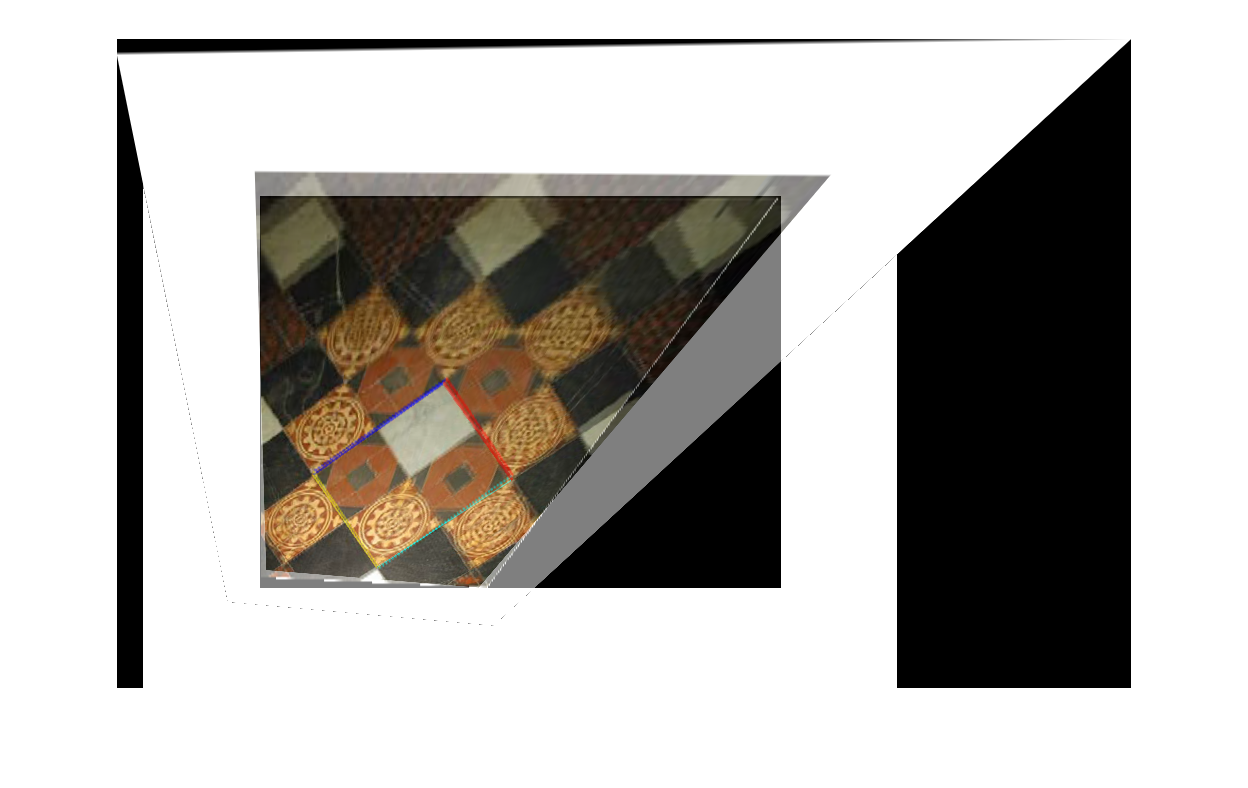
\includegraphics[scale=0.4]{figures/hest.png}
	\caption{Example of warping result.}
\end{figure*}
\begin{itemize}
\item \textbf{task 1}: use \textbf{\textit{main\_homo\_est.m}} to generate simulated $4$ points and use DLT to do homography estimation. Make you function as \textbf{\textit{Hest.m}}.
\item \textbf{task 2}: Once you have done, uncomment the block \textbf{\textit{task 2}} in \textbf{\textit{main\_homo\_est.m}} and try you code usingr real images. The provided code will load one image and wait for you to click. You just pick the four corners of the colored square. Then there will be another image loaded and you again choose $4$ corners of the colored square. Finally, it will call you \textbf{\textit{Hest}} to estimate the homography and do the image warping.
\end{itemize}



\begin{filecontents*}{normalization.m}
	pbar = mean(p,2);% p: 3xn
	pdiff = p(1:2,:) - repmat(pbar(1:2), 1, n);
	mdist = mean(sqrt(diag(pdiff'*pdiff)));
	scale = sqrt(2)/mdist;
	pnormalized(1:2,:) = scale.*pdiff;
	pnormalized(3,:) = 1;
	T = [scale, 0, -pbar(1)*scale; ...
	0, scale, -pbar(2)*scale; ...
	0,0,1];
\end{filecontents*}

\section{Normalization}
Normalization is a key trick to achieve more stable results when we do estimation towards essential, fundamental, and homography matrix. The principle of normalization is nothing but shifting the coordinates to their center and rescaling the mean distance of each point to the center to $\sqrt{2}$. 
\lstinputlisting{normalization.m}

So what you need to do are as follows:
\begin{enumerate}
	\item Normalize $\mathbf{x}_1$: $\tilde{\mathbf{x}}_1=\mathbf{T}_1\mathbf{x}_1$. Do the same for $\mathbf{x}_2$, $\tilde{\mathbf{x}}_2=\mathbf{T}_2\mathbf{x}_2$.
	\item Estimate hompgraphy $\tilde{\mathbf{H}}$ using $\tilde{\mathbf{x}}_1,\ \tilde{\mathbf{x}}_2$, then $\tilde{\mathbf{x}}_2=\tilde{\mathbf{H}}\tilde{\mathbf{x}}_1$.
	\item Finally, $\mathbf{T}_2\mathbf{x}_2=\tilde{\mathbf{H}}\mathbf{T}_1\mathbf{x}_1 \Rightarrow \mathbf{x}_2 = \mathbf{T}_2^{-1}\tilde{\mathbf{H}}\mathbf{T}_1\mathbf{x}_1 \Rightarrow
	\mathbf{H}=\mathbf{T}_2^{-1}\tilde{\mathbf{H}}\mathbf{T}_1$.
\end{enumerate}

\section{RANSAC}
Recall that RANSAC needs 
\begin{itemize}
	\item minimum set for model fitting: for homography, the minimum set is $4$.
	\item model estimation: your implementation \textbf{Hest.m} (\textcolor{red}{remember to add normalization)}.
	\item a distance metric and threshold to justify the iniliers and outliers: here we use the following criteria:
	since $x_2\approx \mathbf{H}x_1$ and $x_1\approx \mathbf{H}^{-1}x_2$, we setup $\epsilon_i=||x_2-\mathbf{H}x_1||+||x_1-\mathbf{H}^{-1}x_2||$. You can specify a threshold manually right now.
\end{itemize}

\end{document}